\documentclass[border=4pt]{standalone}
\usepackage[T1]{fontenc}
\usepackage{tikz}
\usetikzlibrary{arrows.meta,positioning,fit,backgrounds,shapes.geometric,calc}
\definecolor{orch}{HTML}{234767}
\definecolor{ctx}{HTML}{EAF1F8}
\definecolor{retr}{HTML}{E2F0ED}
\definecolor{ext}{HTML}{F7EBDD}
\definecolor{infra}{HTML}{F1F3F5}
\tikzset{
 every node/.style={font=\sffamily\fontsize{8.5}{10}\selectfont,align=center},
 block/.style={draw=orch!80,fill=white,rounded corners=1.5pt,minimum height=7mm,inner sep=3pt,line width=.55pt},
 context/.style={block,fill=ctx},
 engine/.style={block,fill=orch,text=white},
 retrieval/.style={block,fill=retr},
 external/.style={block,fill=ext},
 storage/.style={block,fill=infra},
 flow/.style={-{Stealth[length=2mm]},draw=orch!90,line width=.65pt},
 control/.style={flow,dashed},
 error/.style={flow,densely dotted},
 group/.style={draw=orch!50,rounded corners=3pt,inner sep=5pt,line width=.5pt},
 heading/.style={font=\sffamily\bfseries\fontsize{8.5}{10}\selectfont,text=orch},
 edgelabel/.style={font=\sffamily\fontsize{7.5}{9}\selectfont,fill=white,inner sep=1pt,text=orch}
}

\begin{document}
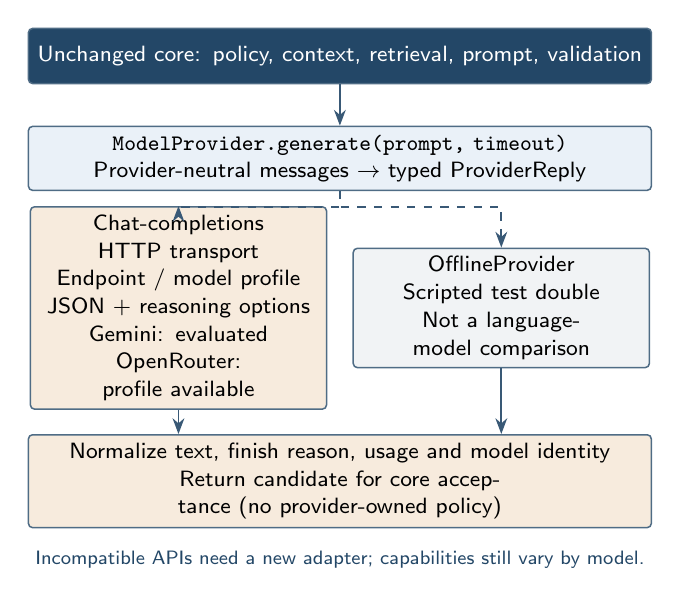
\begin{tikzpicture}
\node[engine,text width=7.7cm] (core) at (0,0) {Unchanged core: policy, context, retrieval, prompt, validation};
\node[context,text width=7.7cm] (contract) at (0,-1.3) {\texttt{ModelProvider.generate(prompt, timeout)}\\Provider-neutral messages $\rightarrow$ typed ProviderReply};
\node[external,text width=3.55cm] (http) at (-2.05,-3.2) {Chat-completions HTTP transport\\Endpoint / model profile\\JSON + reasoning options\\Gemini: evaluated\\OpenRouter: profile available};
\node[storage,text width=3.55cm] (fake) at (2.05,-3.2) {OfflineProvider\\Scripted test double\\Not a language-model comparison};
\node[external,text width=7.7cm] (normal) at (0,-5.4) {Normalize text, finish reason, usage and model identity\\Return candidate for core acceptance (no provider-owned policy)};
\draw[flow] (core) -- (contract);
\draw[control] (contract.south) -- ++(0,-.2) -| (http.north);
\draw[control] (contract.south) -- ++(0,-.2) -| (fake.north);
\draw[flow] (http) -- (http|-normal.north);
\draw[flow] (fake) -- (fake|-normal.north);
\node[edgelabel] at (0,-6.4) {Incompatible APIs need a new adapter; capabilities still vary by model.};
\end{tikzpicture}
\end{document}
